\documentclass{beamer}

\usepackage{listings}
\usepackage{color}
\usepackage{hyperref}



\begin{document}

\begin{frame}
\frametitle{CS24420 \& MA25220 \& MT25220 \& MX35220 \& CSM0120}

\begin{center}
\begin{huge}
Lecture 1: Introduction 
\end{huge}
\bigskip

Amanda Clare (afc@aber.ac.uk)

\end{center}
\end{frame}

\begin{frame}
\frametitle{Modules}
\begin{itemize}
\item CS24420 - Scientific Python
\item MA25220 - Introduction to Numerical Analysis and its
  Applications
\item MT25220 - Cyflwyniad i Ddadansoddiad Rhifiadol a'i gymhwysiadau
\item MX35220 - Introduction to Numerical Analysis and its Applications
\item CSM0120 - Python for Scientists
\end{itemize}
\end{frame}

\begin{frame}
\frametitle{What programming have you done?}

What programming have you done so far? 

\bigskip

UKIEPC on Sat 29th Oct?

\end{frame}


\begin{frame}
\frametitle{Times}
\begin{itemize}
\item Module content on Blackboard.
\item 2 lectures and a practical each week (all compulsory).
\begin{itemize}
\item Tues 4:10pm A6 - lecture
\item Tues 5:10pm B23 - prac
\item Friday 13:10pm B23 - lecture 
\end{itemize}
\item Work week in week beginning 14th November 
\item Module coordinators: Amanda Clare (afc), Tudur Davies (itd)
\item Some lectures given by Sam Nicholls (msn)
\end{itemize}
\end{frame}

\begin{frame}
\frametitle{Assessments}
Different assessments:
\begin{itemize}
\item CS24420: 30\% worksheets, 70\% exam
\item MA25220/MT25220/MX35220: 30\% worksheets, 20\% assignments, 50\% exam
\item CSM0120: 2 assignments (40\%, 60\%) 
\end{itemize}
\end{frame}

\begin{frame}
\frametitle{Worksheets}
\begin{itemize}
\item One every week, including today.
\item Graded 0, 1, 2.
\item Signed off by demonstrators.
\item You have a maximum of 3 practical sessions (15 days) for each
  worksheet, before it gets a 0.
\item Do the worksheet during the practical. If you need more time, do
  it at home or in B23 (24 hours). 
\item You can get the worksheet signed off in the current prac, or the
  next prac, or the one after. But not after that.
\item Any problems (sickness etc), see me.
\end{itemize}
\end{frame}


\begin{frame}
\frametitle{Books}
\begin{itemize}
\item Automate the Boring Stuff with Python, Al Sweigart 
    \url{https://automatetheboringstuff.com/\#toc}
\item Many other Python books in library and in bookshops
\item See recommendations on Blackboard
\end{itemize}
\end{frame}

\begin{frame}
\frametitle{Python creation}
\begin{itemize}
\item First created in 1989 by Guido van Rossum
\item Named after comedy TV show Monty Python's Flying Circus
\item Owned by the Python Software Foundation (PSF), a non-profit org
\item van Rossum is 'Benevolent Dictator For Life'
\item van Rossum has worked for Google, now works for Dropbox
\end{itemize}
\end{frame}



\begin{frame}
\frametitle{Topics for Semester 1}
\begin{itemize}
\item Language basics
\item Data structures
\item NumPy
\item Functions
\item Organising code
\item Objects
\item File handling
\item Plotting
\end{itemize}
\end{frame}

\begin{frame}
\frametitle{Topics for Semester 2}
\begin{itemize}
\item CS24420 - Science, noise, statistics, hot topics
\item MA25220/MT25220/MX35220 - Numerical approximations to maths problems
\item CSM0120 - First semester only, but maybe extra database material
  towards end of module.
\end{itemize}
\end{frame}



\begin{frame}
\frametitle{Python 2 vs Python 3}
\begin{itemize}
\item There are two versions of Python in active use in industry.
\item Although Python 3 has been around for many years, legacy code
  and libraries
  have been slow to move.
\item This course will mention the differences as we come across them.
\end{itemize}
\end{frame}

\begin{frame}
\frametitle{Python home}
\begin{itemize}
\item \url{http://www.python.org}
\item Python 3.5 or Python 2.7
\item Language reference: \url{http://docs.python.org/3/reference}
\item Library reference: \url{http://docs.python.org/3/library}
\end{itemize}
\end{frame}


\begin{frame}
\frametitle{Style of Python}
\begin{itemize}
\item Scripting, OO, functional, imperative.
\item Dynamic.
\item Get things done quickly (perhaps not always correctly).
\item Many libraries.
\item Large community, lots of cheap books and example code.
\item Uses whitespace to indicate code structure.
\end{itemize}
\end{frame}


\begin{frame}
\frametitle{Anaconda, libraries and scientific python}
\begin{itemize}
\item Many libraries are bundled with Python.
\item Some scientific libraries are not.
\item To easily install Python with scientific libraries on Mac or Windows, try the
  Anaconda distribution (\url{https://www.continuum.io/downloads})
\item Installation help in the practical, next.
\end{itemize}
\end{frame}


\begin{frame}
\begin{center}
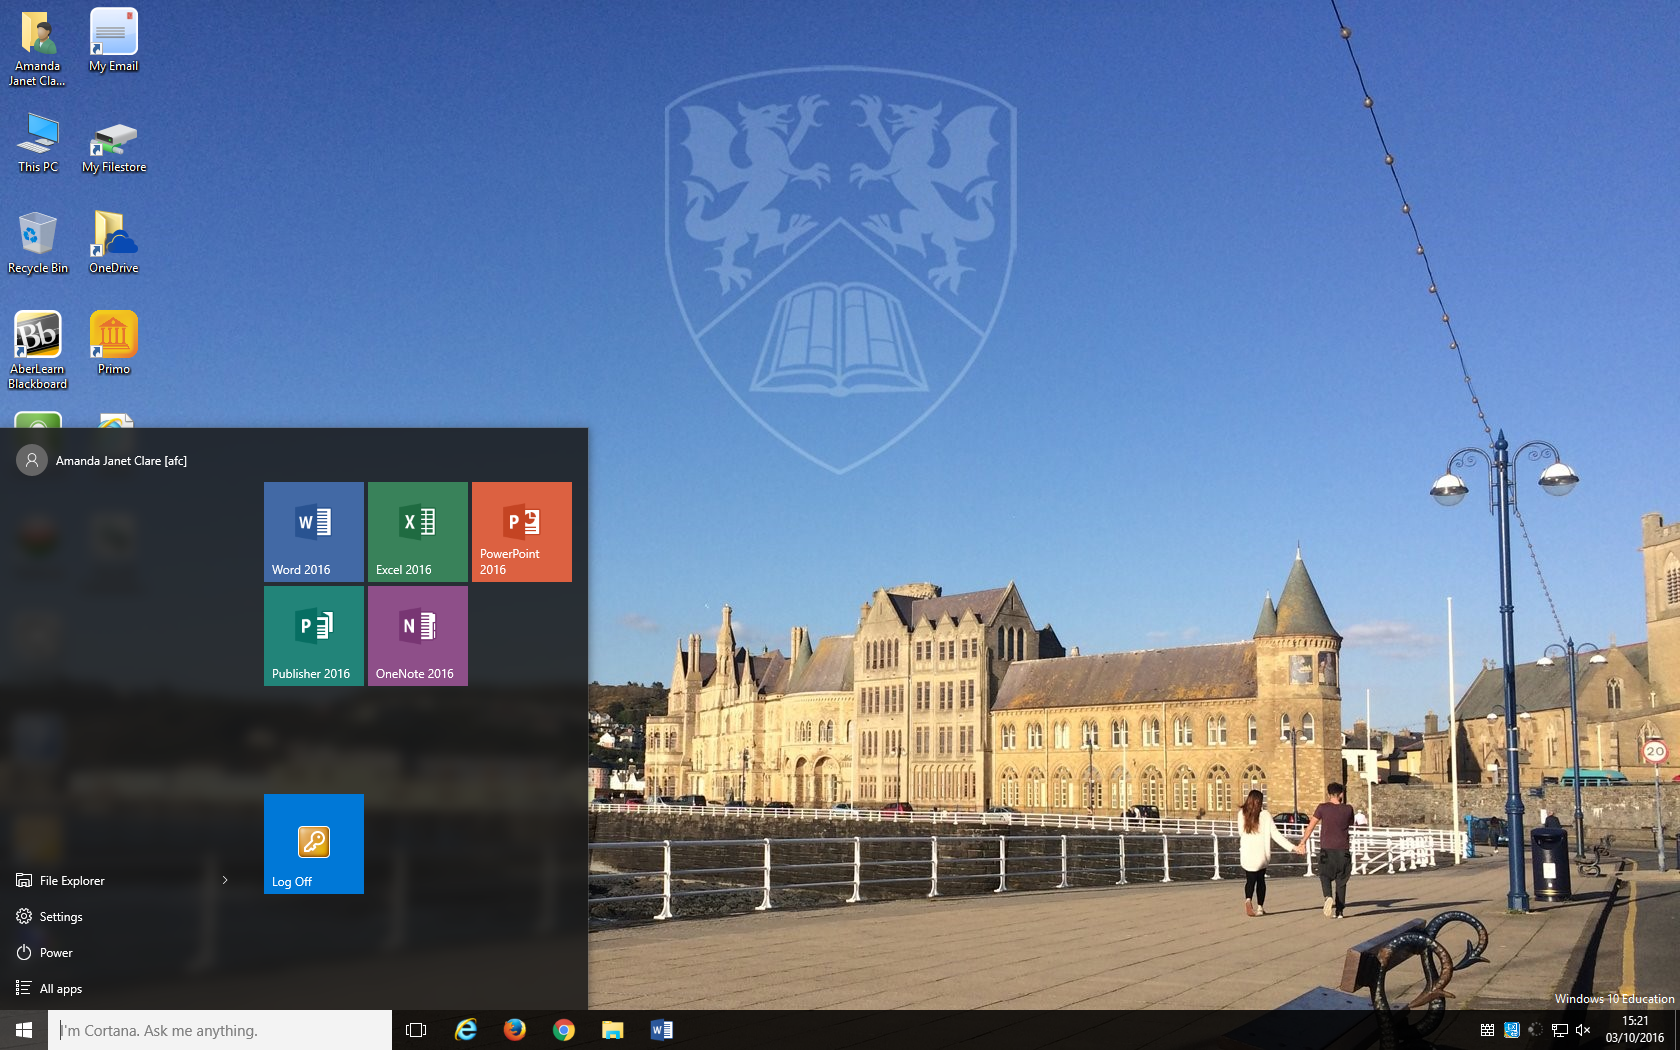
\includegraphics[width=10cm]{windows10.png}
\end{center}
\end{frame}

\begin{frame}
\begin{center}
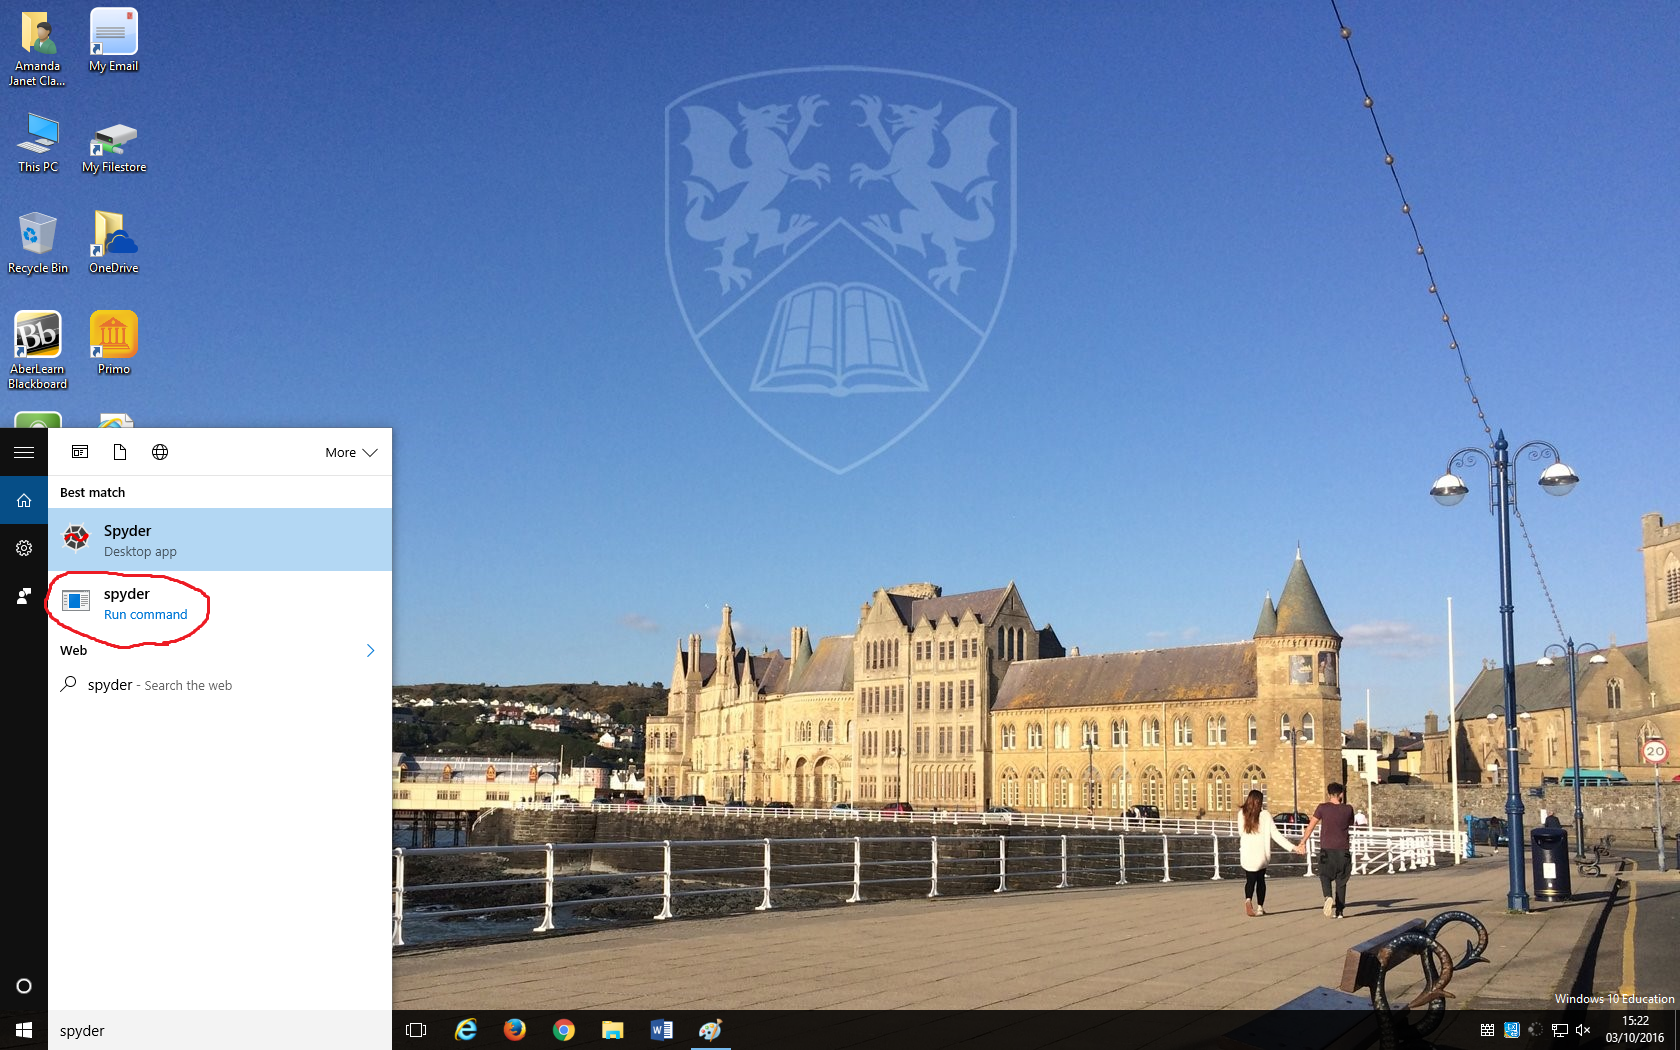
\includegraphics[width=10cm]{choosespyder.png}
\end{center}
\end{frame}


\begin{frame}
\frametitle{Editors, IDES, consoles}
\begin{itemize}
\item gedit/aquamacs/vim/emacs/notepad++ 
\item Spyder IDE
\end{itemize}
\end{frame}

\begin{frame}
\frametitle{Running the code}
\begin{itemize}
\item Python: do we mean the language specification, or an implementation of an
  environment to run Python code.
\item We'll be using CPython to run code (but you'll see this just as ``python'').
\item Interactive console vs iPython vs coding in files/modules.
\item Python code is usually compiled to byte code then run on a virtual
  machine. CPython does both.  Jython will compile Python bytecode for
  running on the JVM (only v2.7).
\item But it will feel like it's interpreted, as the bytecode is
  interpreted. 
\item You will see that bytecode-compiled .pyc files are made
  from your .py files.
\end{itemize}
\end{frame}


\begin{frame}
\frametitle{Consoles/REPLs}
\begin{itemize}
\item Interactive prompt to try out code (REPL - read-evaluate-print
  loop)
\item Python console 
\item iPython console
\end{itemize}
\end{frame}


\begin{frame}
\frametitle{Spyder}
\begin{itemize}
\item Pros and cons of an IDE, vs editor plus console
\item Try it and see what you think
\end{itemize}
\end{frame}




\begin{frame}
\frametitle{Let's get setup/installed}
\begin{itemize}
\item Worksheet 1 starts today
\item In B23 at 5:10 today to ensure your uni setup is good 
\item And to install it on your laptops if wanted.
\end{itemize}
\end{frame}


\end{document}
